\documentclass[twocolumn]{article}
\usepackage{epsfig}
\usepackage{psfig}
\usepackage{graphicx}
\usepackage{url}
\usepackage{times}
\usepackage{amsmath}
\usepackage{paralist}
\usepackage[colorlinks,linkcolor=red,anchorcolor=blue,citecolor=green]{hyperref}
\setlength{\columnsep}{20pt}
\newcommand{\SA}{Simulated Annealing~}
\makeatletter
\def\verbatim{\small\@verbatim \frenchspacing\@vobeyspaces \@xverbatim}
\makeatother
\begin{document}

\title{{\bf The Application of Simulated Annealing in Polynomial Solver}\\ }

\author{Xin Wang\\ \vspace{0.5cm}\\
 10302010023}

\date{}
\maketitle
\begin{abstract}
\SA is a widely-adopted physical computing algorithm, which is a suitable candidate to estimate the extreme point of a cost function. This paper proposes two versions of Simulated Annealing Solver to polynomial extreme points implemented in floating point number and fixed point number respectively. Moreover, I give the execution statistics of both two versions and the error rate of the fixed point one to explore the potential of performance increase.
\end{abstract}

\section{Introduction}
\label{sec:intro}
\SA is a typical natural computing algorithm whose name is inspired from  annealing in metallurgy, a technique involving heating and controlled cooling of a material to increase the size of its crystals and reduce their defects, both are attributes of the material that depend on its thermodynamic free energy. \SA is a generic probabilistic meta-heuristic for the global optimization problem of locating a good approximation to the global optimum of a given function in a large search space. It is widely used when search space is discrete. For certain problems, simulated annealing may be more efficient than exhaustive enumeration provided that the goal is merely to find an acceptably good solution in a fixed amount of time, rather than the best possible solution. In engineering and scientific calculation, \SA is frequently adopted in network traffic engineering~\cite{Pasias:2004}, environmental science~\cite{Jingwen:2009}, sensor network~\cite{Zimmerman:2007}, EDA placement design~\cite{Naifeng:2011}, etc. Within these domains, \SA is widely adopted for its stochastic way of addressing the global optimal in a given range, which could save much computational resource while the precision is controllable and sufficient for the engineering requirements.

Given the fact that \SA is suitable for determining an optimal solution with tolerable error rate, it would be efficient to calculate the near optimum solution in polynomial equation with determined range. As a matter of fact, both \SA and Genetic Algorithm are frequently-used approaches in searching the global optimal solution in linear algebra problems~\cite{Chen:1998} based on their capability to estimate the near optimal solution of liner polynomial equations and this would be a hotspot in future research.

This paper attempts to implement a polynomial equation solver based on \SA approach. I define a series of input data sets with different sizes and computation loads to comprise a benchmark dataset. Then, considering the real-time running environments, I evaluate the \SA polynomial solver using several code instrument tools and performance analysers to illustrate the workload of \SA solver. Furthermore, given that the polynomial solver problems are often defined in real number domain while the floating point operation is one of the most time-consuming and power-cost part in a computation-intensive program~\cite{DaiChen:2013}, I also implement the comparing version using fixed point units and explore the performance increase and the sacrifice of accuracy in order to make trade-offs between performance and accuracy.

The rest of this paper is organized as follows, Section~\ref{sec:related} relates the background knowledge and related work of \SA solvers. Section~\ref{sec:design} elaborates the design of the proposed \SA solver including the data format, usage, parameters, and the fixed-point version for comparison. Section~\ref{sec:experiment} presents the experimental statistics and analyzes the results. Section~\ref{sec:discussion} discusses the insights attained from the experiments and proposes some suggestions for optimization. Finally, Section~\ref{sec:conclusion} draws the conclusion of this paper. 

\section{Related Work}
\label{sec:related}
\subsection{Mechanism of \SA}
As is mentioned in Section~\ref{sec:intro}, \SA algorithm is inspired from the natural process of gradual cooling of a melted solid to obtain the minimum energy value. This energy is equivalent to the objective function value in a conventional optimization problem.

Generally, \SA algorithm consists of three operations: generation, acceptance and cooling. Similar to genetic algorithm, \SA also includes the concept of generation. The generation operation changes the current solution $x$ and generates the next solution $x'$ using a probability distribution known as Maxwell-Boltzmann distribution. The acceptance operation decides whether the temperature change is acceptable. The acceptance is determined from the difference $\Delta E = E'-E$ of the current energy $\Delta E = f(x)$ and the energy of the next solution $\Delta E = f(x')$ as well as the temperature parameter T. The simplified algorithm shown in Equation~\ref{eq:SA_prob} provides a efficient simulation of the Boltzmann distribution~\cite{Hiroyasu:2010}.

\begin{equation}
\label{eq:SA_prob}
P=
\begin{cases}
1 & if(\Delta E < 0) \\
e^{-\frac{\Delta E}{T}}&otherwise \\
\end{cases}
\end{equation}

Firstly, the change is acceptable if $\Delta E < 0$, otherwise the change would be accepted according to a certain probability. The cooling operation generates the temperature of the next state from the temperature with the decreasing coefficient defined by a constant $\lambda$. From the equation we could observe that the probability decreases with the lowering of temperature. Thus at the beginning of the simulation, both the temperature and the probability of accepting a higher energy are high, correspondent with the natural process of cooling a melted metal. The probability of accepting a higher energy state is vital to the \SA simulation since the fundamental of \SA algorithm is to jump out of local optimal point~\cite{Garcia:2009} and find the global optimal solution.
\subsection{Existing \SA Solvers}
\SA solvers exist widely in scientific and engineering domain to search for the optimal solution of problem related to linear algebra. The most pervasive \SA solver is the Adaptive Simulates Annealing (ASA) developed by Lester Ingber et al.~\cite{Lester:2013}. ASA is a C-language code developed to statistically find the best global fit of a nonlinear constrained non-convex cost-function over a D-dimensional space. Yet ASA is an integrated toolset for general usage and users need to change the source code and recompile the entire program when they need to solve their own problems. Matlab mathematical software also provides some tiny toolboxes for \SA solvers, some of them concentrate on polynomial equation solver~\cite{Matlab:2009} based on stochastic search in linear algebra space yet these toolsets are developed in Matlab language and could only run under the framework of Matlab software. 

\section{Design}
\label{sec:design}
\subsection{Solver Overview}
The \SA polynomial solver is implemented in ANSI C language under GNU/Linux system with total 146 lines of code. The solver reads the input data from text files including the coefficients of the polynomial equations and calculate the optimal solution (extreme point) of each equation using \SA with given initial and final temperature. The result of each equation would be recorded in the output files.
\subsection{Input Data}
A typical record in the input data file is like this:
$$[-9397.819, 602.181] -799.515 -687.799 -411.936$$
The two numbers in the brackets define the domain of the extreme point, i.e. the solver would only search the optimal solution within this domain. The following several numbers define the coefficients in descending order. For instance, the record above indicates an equation of:
$$f(x) = -799.515x^2-687.799x-411.936$$
where $x\in[-9397.819, 602.181]$. Similarly, the format of the output is like this:
$$x = -0.986, cost(x) = -2.928e+03$$
This means the optimal solution and the corresponding cost of the function.
\subsection{Parameters}
The usage of the main program is as follows:
\begin{verbatim}
./anneal <input_file> <output_file> 
  [--options]
\end{verbatim}
The meaning of each domain is explained as follows:
\begin{compactitem}
\item input\_file: Path of the input data file
\item output\_file: Path of the output data file
\item options: Optional parameters of the program including
    \begin{compactitem}
    \item ini\_temp: The initial temperature; default value is 1000.
    \item fin\_temp: The final temperature; default value is 5e-5.
    \item lambda: The coefficient of temperature decrease; default value is 0.7.
    \end{compactitem}
\end{compactitem}
\subsection{Comparing Version}
As a fixed-point version for comparison, I substitute the floating point operations in the \SA solver by fixed-point ones and adjust the bits of decimal part. The input data is the same with floating point ones while the output result would be evaluated according to the criteria that would be introduced in Section~\ref{sec:comparison}. 

\section{Experiment and Analysis}
\label{sec:experiment}
The following experiment will measure several architectural-independent metrics of \SA solver and evaluate the architectural characteristics. Section~\ref{sec:setup} will introduce the experiment environment first. The experiment would be classified into three categories: Section~\ref{sec:computation} analyzes the computation resource related metrics including various instruction ratio, branch misprediction rate, floating point operation ratio, etc. Section~\ref{sec:memory} presents the result of memory footprint including the memory utilization, memory-related instruction ratio and cache miss rate. Section~\ref{sec:comparison} will make comparison of the two versions of \SA solvers with respect to the decrease of accuracy and the change of performance.
\subsection{Experiment Setup}
\label{sec:setup}
The experiment is carried out by a C-language \SA solver under 32-bit GNU/Linux 2.6.43. The CPU is Intel Core i7-2600@3.40GHz with 4 cores. L1 cache includes a 4 $\times$ 32 KB instruction cache and 4 $\times$ 32 KB data cache. L2 cache is 4 $\times$ 256 KB while the shared L3 cache is 8 MB. The input data sets were generated randomly and classified into three categories according to different sizes as in Table~\ref{tab:sizes}.

\begin{table}
  \centering
  \begin{tabular}{|l|l|l|}\hline
  \textbf{Data Set} & \textbf{Text file size} & \textbf{Number of equations}\\\hline
  Small & 19KB & 128 \\\hline
  Middle&127KB&512\\\hline
  Large&148KB&1024\\\hline
  \end{tabular}
  \caption{Size of different data sets}\label{tab:sizes}
\end{table}

\subsection{Computation Resource}
\label{sec:computation}
Computation Resource includes the ratio of different kind of instructions as well as other categories of CPU-related metrics such as memory/branch instruction ratios, branch misprediction rate under different prediction strategies etc. This part of metrics are measured by the binary instrument framework Pin-Tool and the performance evaluation tools VTune Amplifier provided by Intel. The following statistics are collected by running the solver using the different data sets except where noted.
\subsubsection{Instruction Ratio}
In this part I measure the ratio of memory and branch related instructions to reveal the effect of jump/branch instructions to the overall performance. The statistics is shown in the Figure~\ref{fig:ratio}. From the graph we could observe that the memory ratio is at a high level($>=40\%$) while the branch-related instructions take about 20\% of the overall instructions. This phenomenon could be ascribed to the frequent condition judgement of temperature change. High percentage of memory/branch instructions require the processor to be more efficient on branch prediction and memory access bandwidth optimization.

\begin{figure}
\centering
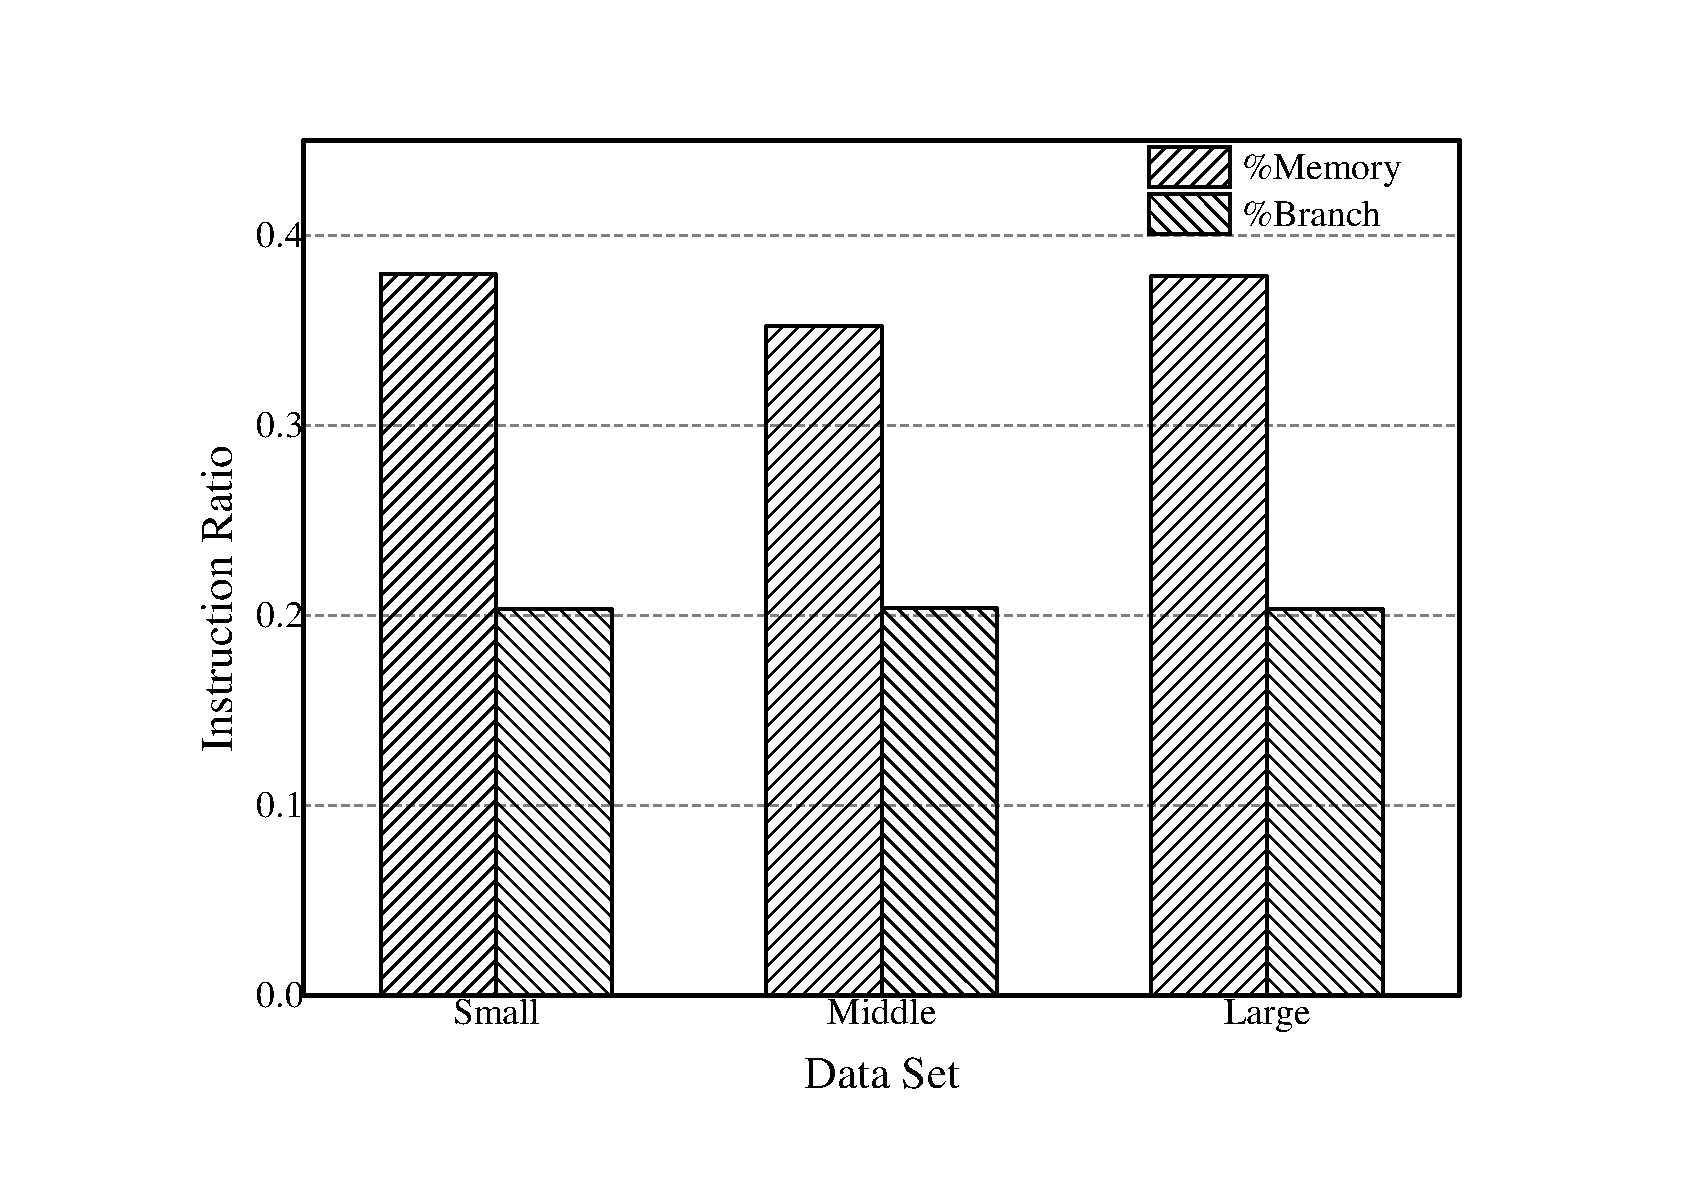
\includegraphics[width=0.50\textwidth]{graph/ins_ratio.pdf}
\caption{Instruction Ratio.}
\label{fig:ratio}
\end{figure}

\subsubsection{IPC and MPC}
In order to excavate the parallelism potential of the \SA solver, I measured the instruction-level parallelism (ILP) and memory-level parallelism (MLP) which are revealed by instruction per cycle (IPC) and memory access per cycle (MPC) respectively. The result is shown in Figure~\ref{fig:ipc_mpc}, from which we could find that the both the IPC and MPC are maintained at a low level. The low level of parallelism indicates that the \SA solvers could be transplanted into in-order processors to save the extra overhead brought by processors with out-of-order issue units such as branch-misprediction, pipeline hazard and memory access scheduling. 

\begin{figure}
\centering
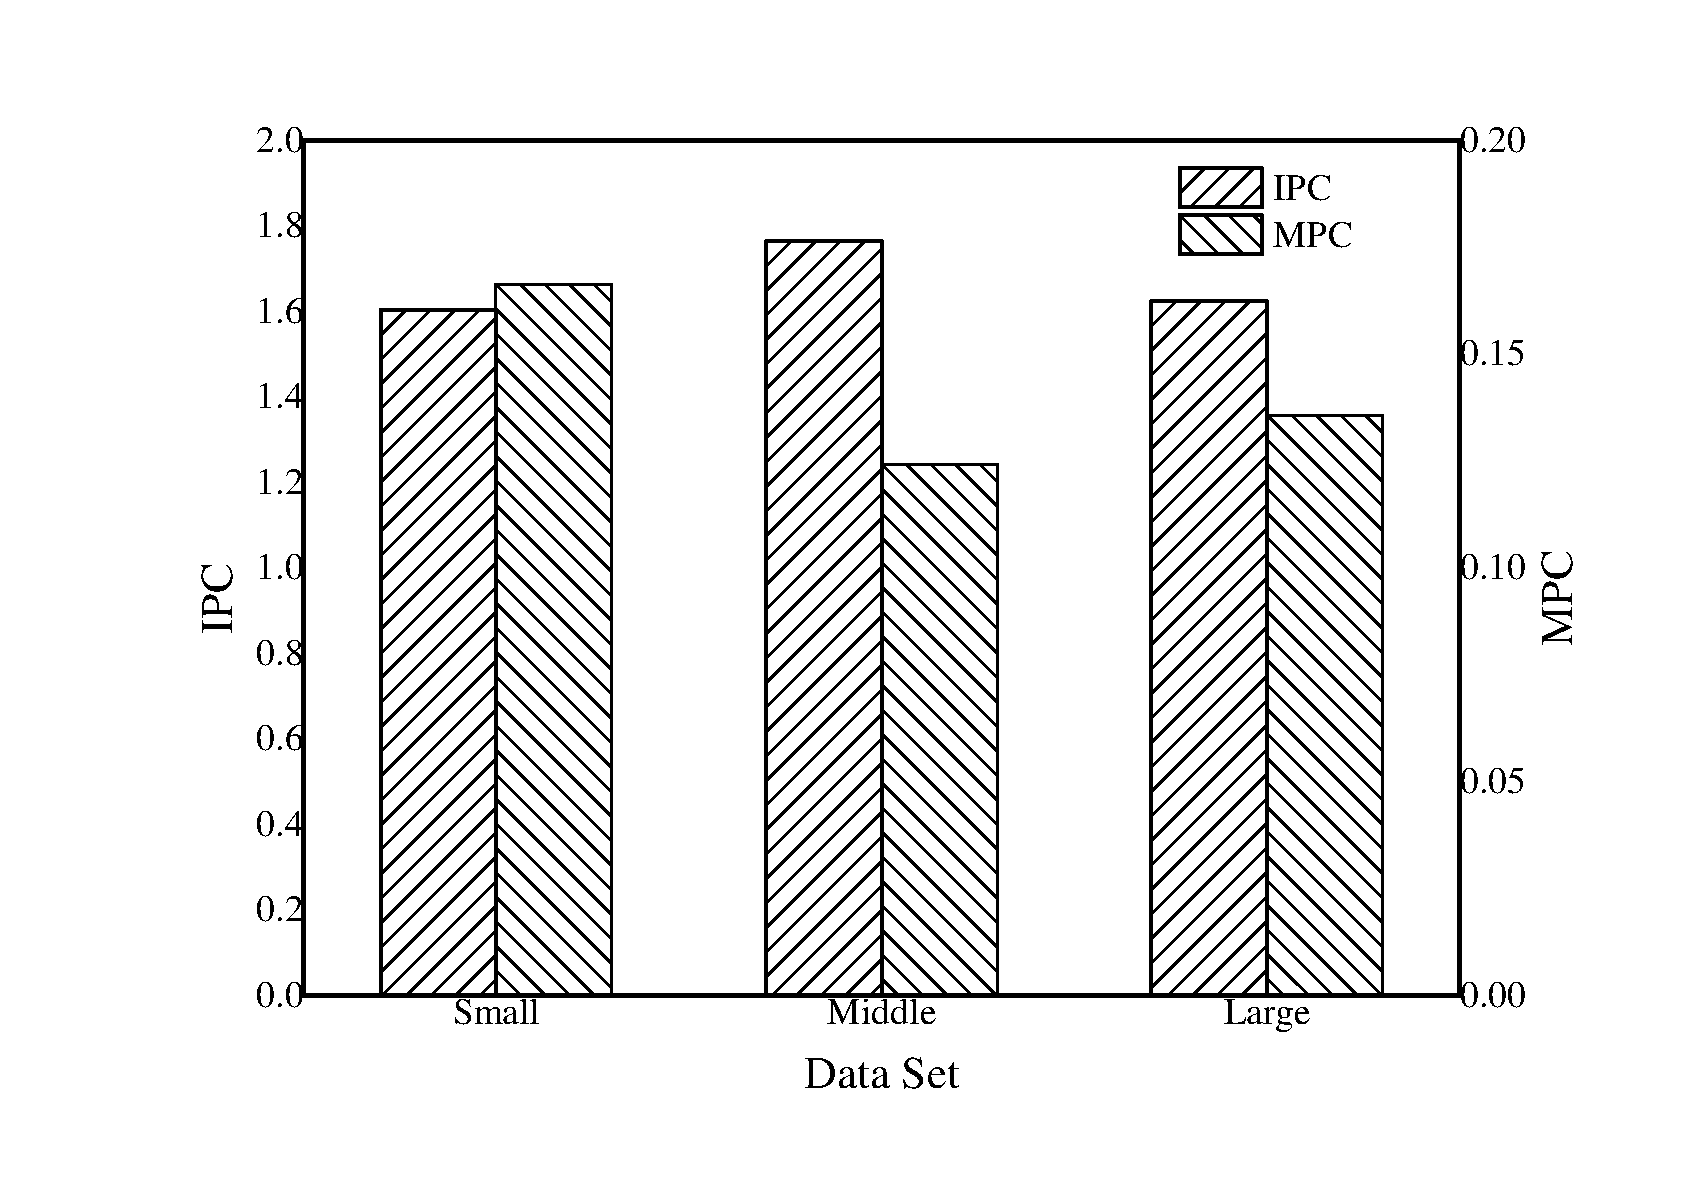
\includegraphics[width=0.50\textwidth]{graph/IPC_MPC.pdf}
\caption{Instruction per Cycle and Memory Access per 1000 Cycles.}
\label{fig:ipc_mpc}
\end{figure}

\subsubsection{IPB}
Instruction per byte of input data (IPB) is an significant metric reflecting computation intensity of a program. I measure the IPB of my solver with three different data sets as well as another two famous benchmark suites: SPECint 2006 and PARSEC for comparison (Thanks to my tutor for SPEC CPU 2006 is a commercial software). 

The logarithm of IPB is plotted in Figure~\ref{fig:IPB}. The curves in the graph show that \SA solver is more computation-intensive than predominant benchmark suites due to frequent random number generation and complicated exponential computation operations. Thus the clock frequency and the performance of ALU still have a significant effect. Moreover, high computation intensity was comprised partially by frequent floating point operations, which would be further discussed in Section~\ref{sec:comparison}.

\begin{figure}
\centering
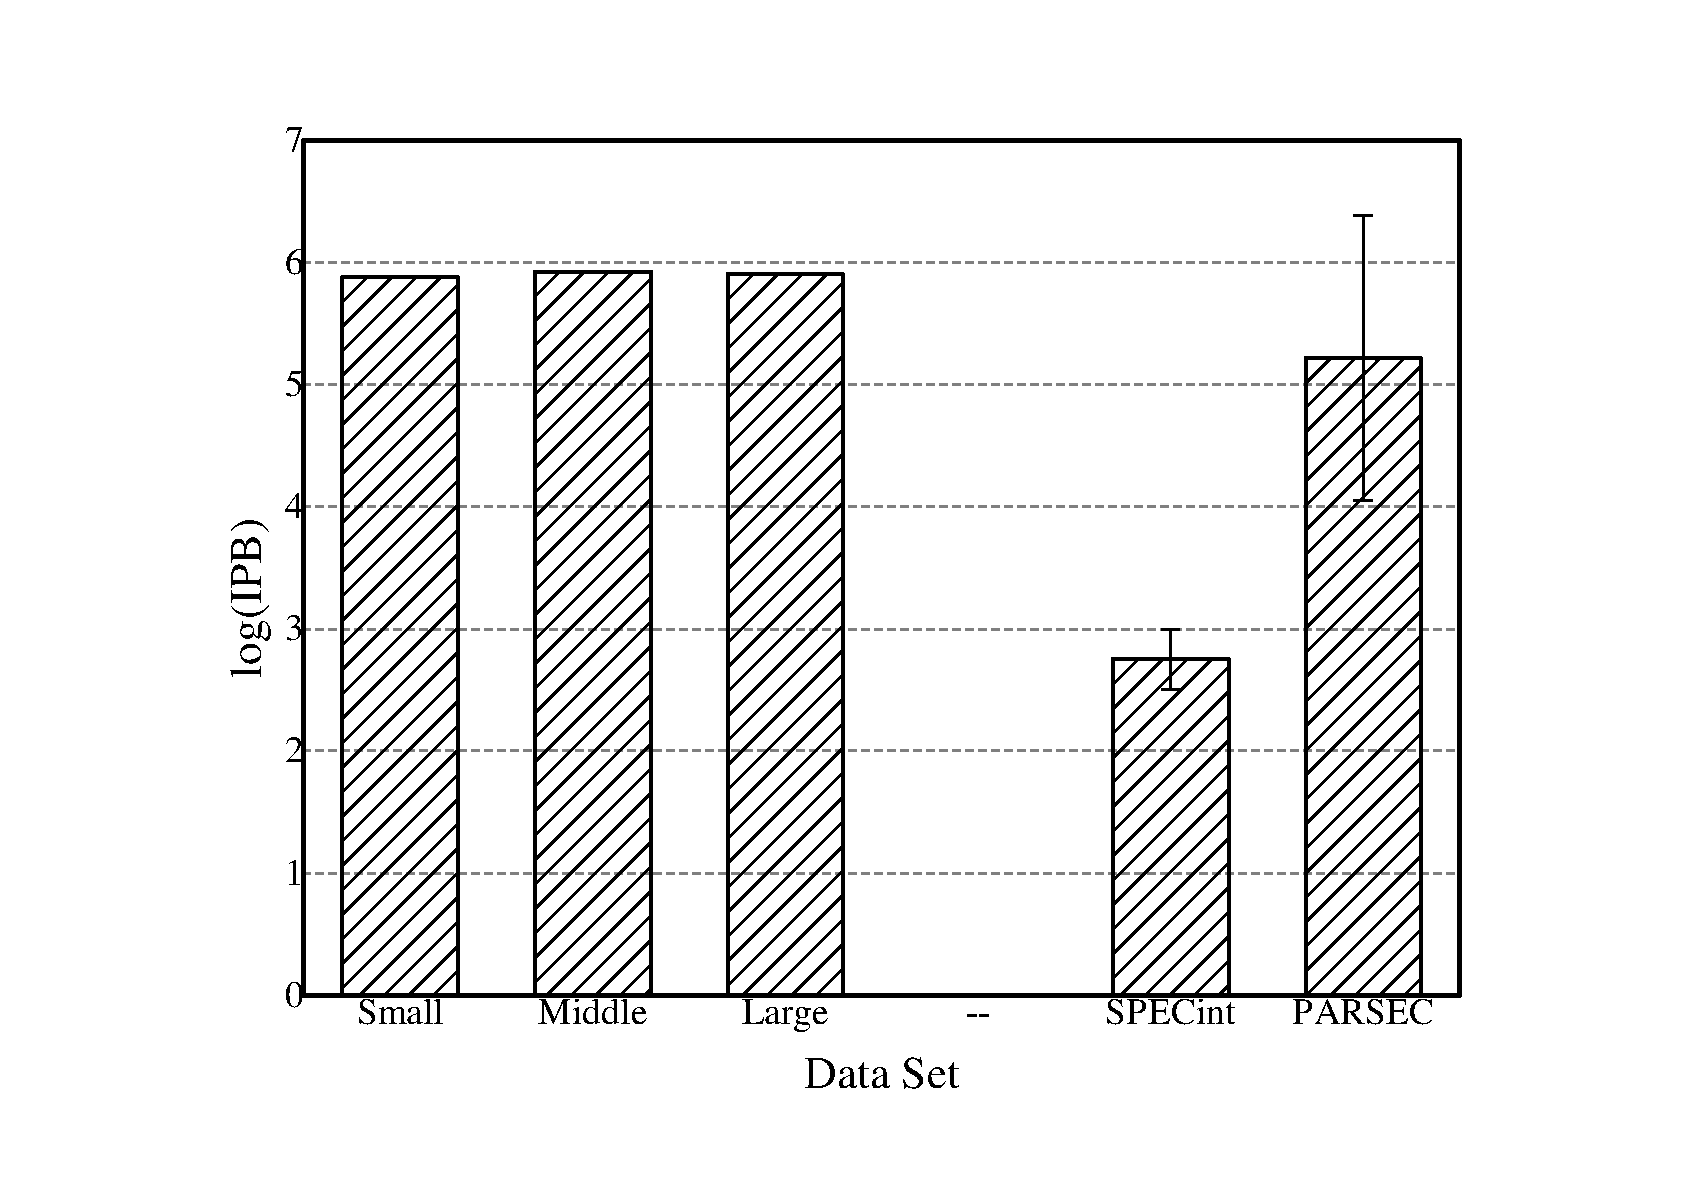
\includegraphics[width=0.50\textwidth]{graph/IPB.pdf}
\caption{Instruction per Byte.}
\label{fig:IPB}
\end{figure}

\subsubsection{Branch Misprediction Ratio }
Branch misprediction is also a significant contributor to stall cycle and slowdown of the instruction. Modern processor chips adopt different prediction strategies to prevent the miss penalty of cache miss. In this experiment we simulate three different prediction algorithms: one-bit, two-bits and two-level strategy and measure the branch misprediction rate respectively.

\begin{compactitem}
\item \textbf{One-bit strategy}: The simplest algorithm of branch prediction. A memory contains a bit indicating whether the branch is recently taken or not.
\item \textbf{Two-bits strategy}: To remedy the shortcoming of one-bit strategy, 2-bit prediction scheme adopts a finite state automata in which a prediction must miss twice before a prediction is changed.
\item \textbf{Two-level strategy}: Branch predictor that use the behavior of other branches to make a prediction called correlating predictors or two-level predictors. Existing correlating predictors add information about the behavior of the most recent branches to decide how to predict a given branch\cite{John:2006,Ribas:2006}.
\end{compactitem}
Figure~\ref{fig:predict} shows the branch misprediction rate under the three strategies. From the graph we could observe that the misprediction rate is a little higher than the average computation intensive programs ($>=0.3$) at simple prediction strategy of one-bit prediction. The misprediction rate decreases notably when more complex prediction algorithm is adopted like two-level strategy. The main part of the program includes a loop of which the condition consists of a randomly generated number thus the branch behavior is much more unpredictable. Considering the branch instruction takes a notable proportion in the overall instructions, more sophisticated branch prediction strategy should be adopted in the architectural design. 

\begin{figure}
\centering
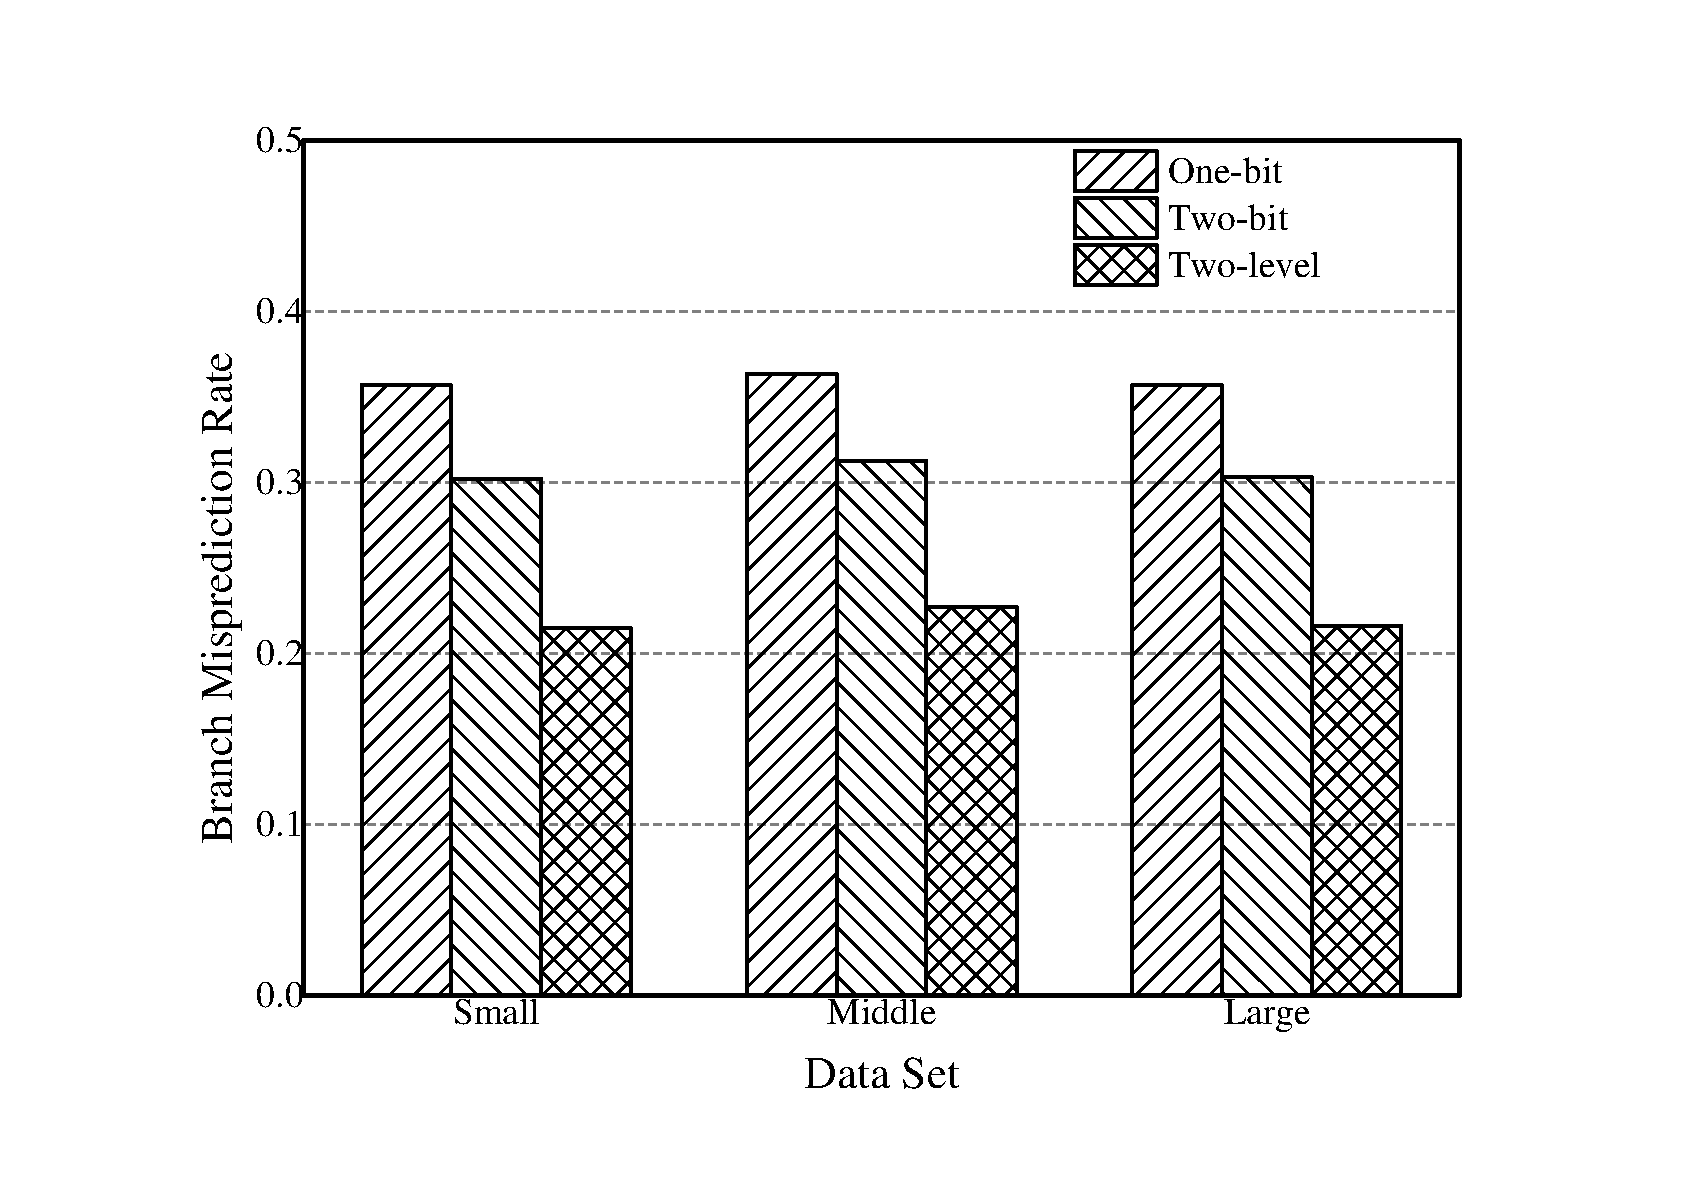
\includegraphics[width=0.50\textwidth]{graph/predict.pdf}
\caption{Branch Misprediction Rate under Different Prediction Strategies.}
\label{fig:predict}
\end{figure}

\subsection{Memory Footprint}
\label{sec:memory}
The memory footprint is also a significant criterion of our program. We leverage the API provided by Intel Pin tools to conduct a series of experiments focused on memory-related behaviors. The metrics measured includes memory usage, cache miss rate, Lest-level Cache (LLC) miss rate under different sizes of LLC.

\subsubsection{Memory Utilization}
I measured the memory usage of resident set size (RSS) of the program using the GNU tool /usr/bin/time. The maximum memory usage of RSS doesn't vary a lot among the three sets of input data and the average value is about 580KB. Considering the input file is text-based files, the small amount of memory usage could be ascribed to the I/O cache optimization while the main loop of the solver does not involve much memory access operations. 

\subsubsection{L1 and L2 Cache Miss Rate}
This is another on-chip level metric reflecting the cache coherence of the program. The L1 and L2 on-chip cache miss rate is shown in Figure~\ref{fig:cache_miss}. Since the working set of solver is not very large, the pressure on cache and memory is not as severe as on instruction handling pipeline. Therefore, it is not necessary to enlarge the cache size further.

\begin{figure}
\centering
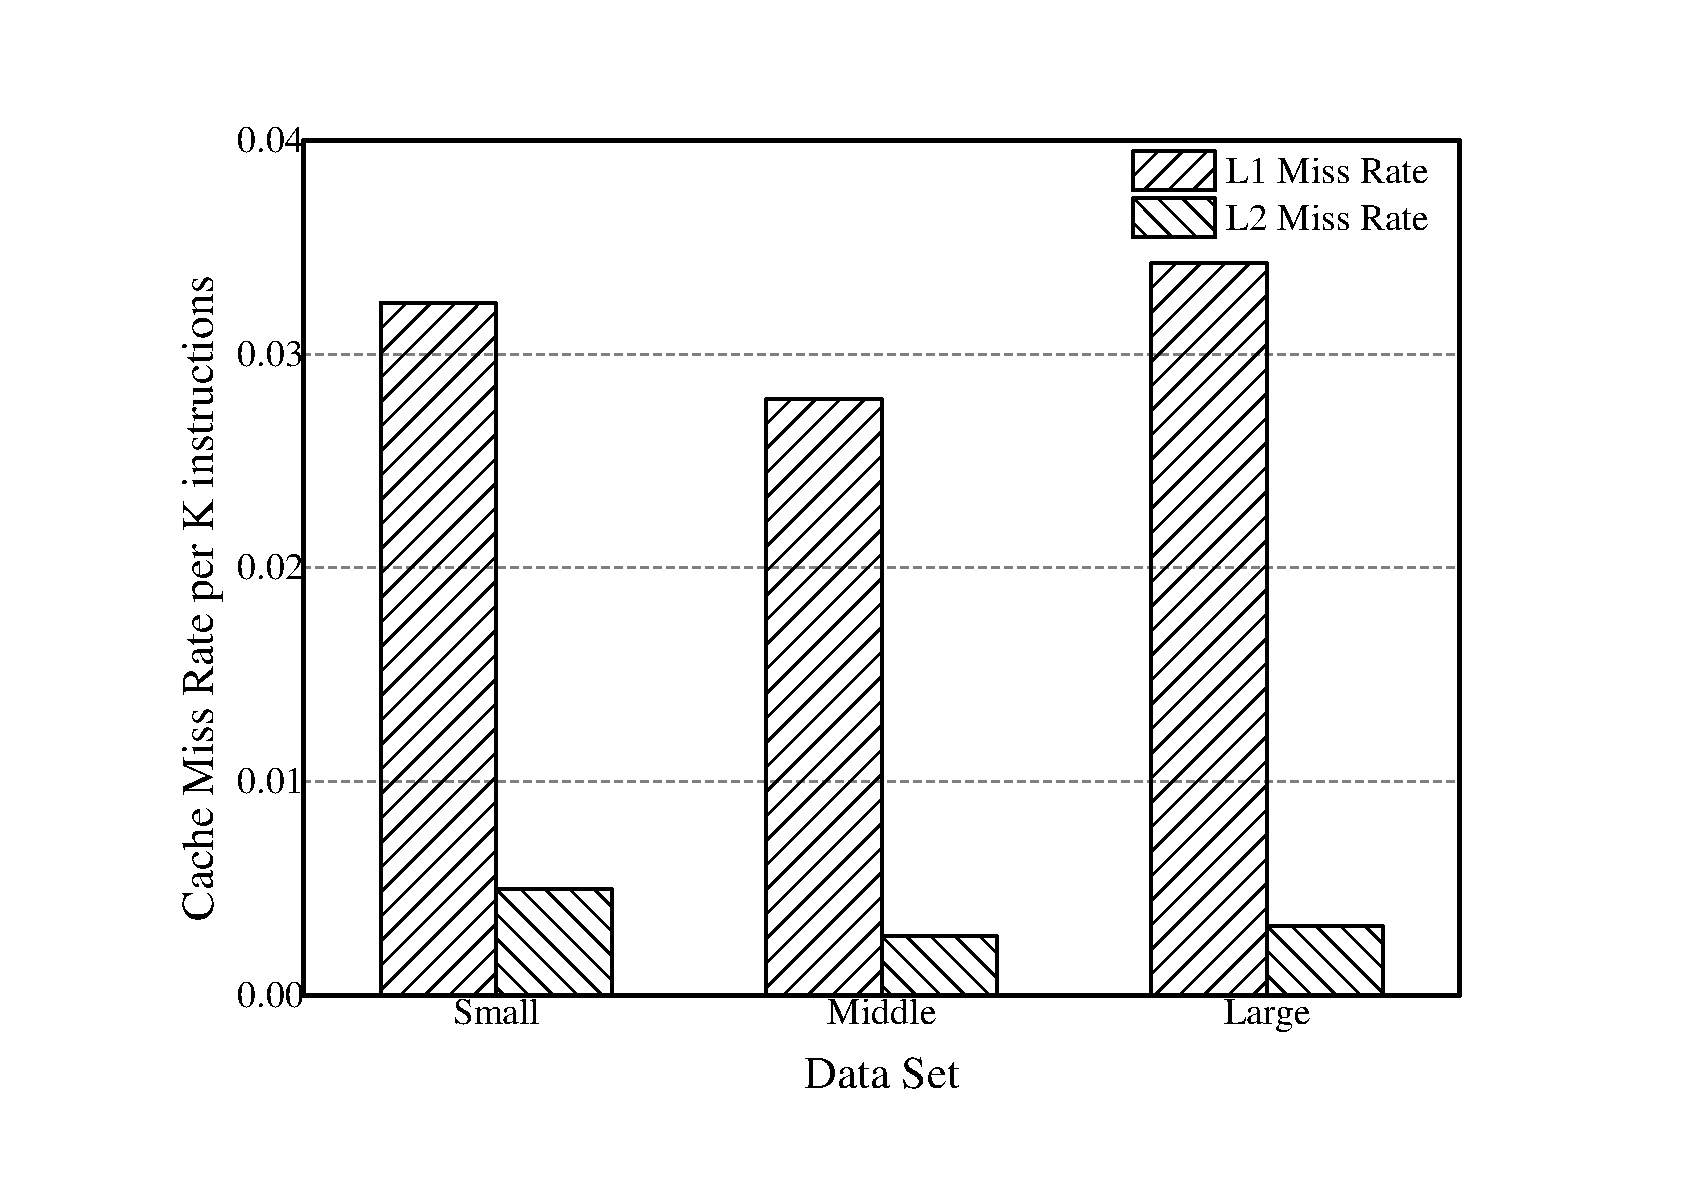
\includegraphics[width=0.50\textwidth]{graph/cache_miss.pdf}
\caption{L1 and L2 Cache Miss Time per K Instructions.}
\label{fig:cache_miss}
\end{figure}

\subsubsection{Last Level Cache Miss Rate}
As to explore the LLC miss rate, we adopt the Cachegring tool integrated in the Valgrind toolset to simulate different size of Last Level Set (LLC) from 1/32MB to 32MB and measure the LLC miss times per 1000 instructions under different sizes of LLC. 

The result is plotted in Figure~\ref{fig:LLC_miss}. The statistics indicate that the LLC miss rate decreases with the increase of LLC size and maintains at a stable level when the LLC size exceeds the working set (1/8MB). Since the working set of the solver is much smaller compared to the size of CPU shared LLC (8MB), the current LLC could generally satisfy the requirement of the solver.
\begin{figure}
\centering
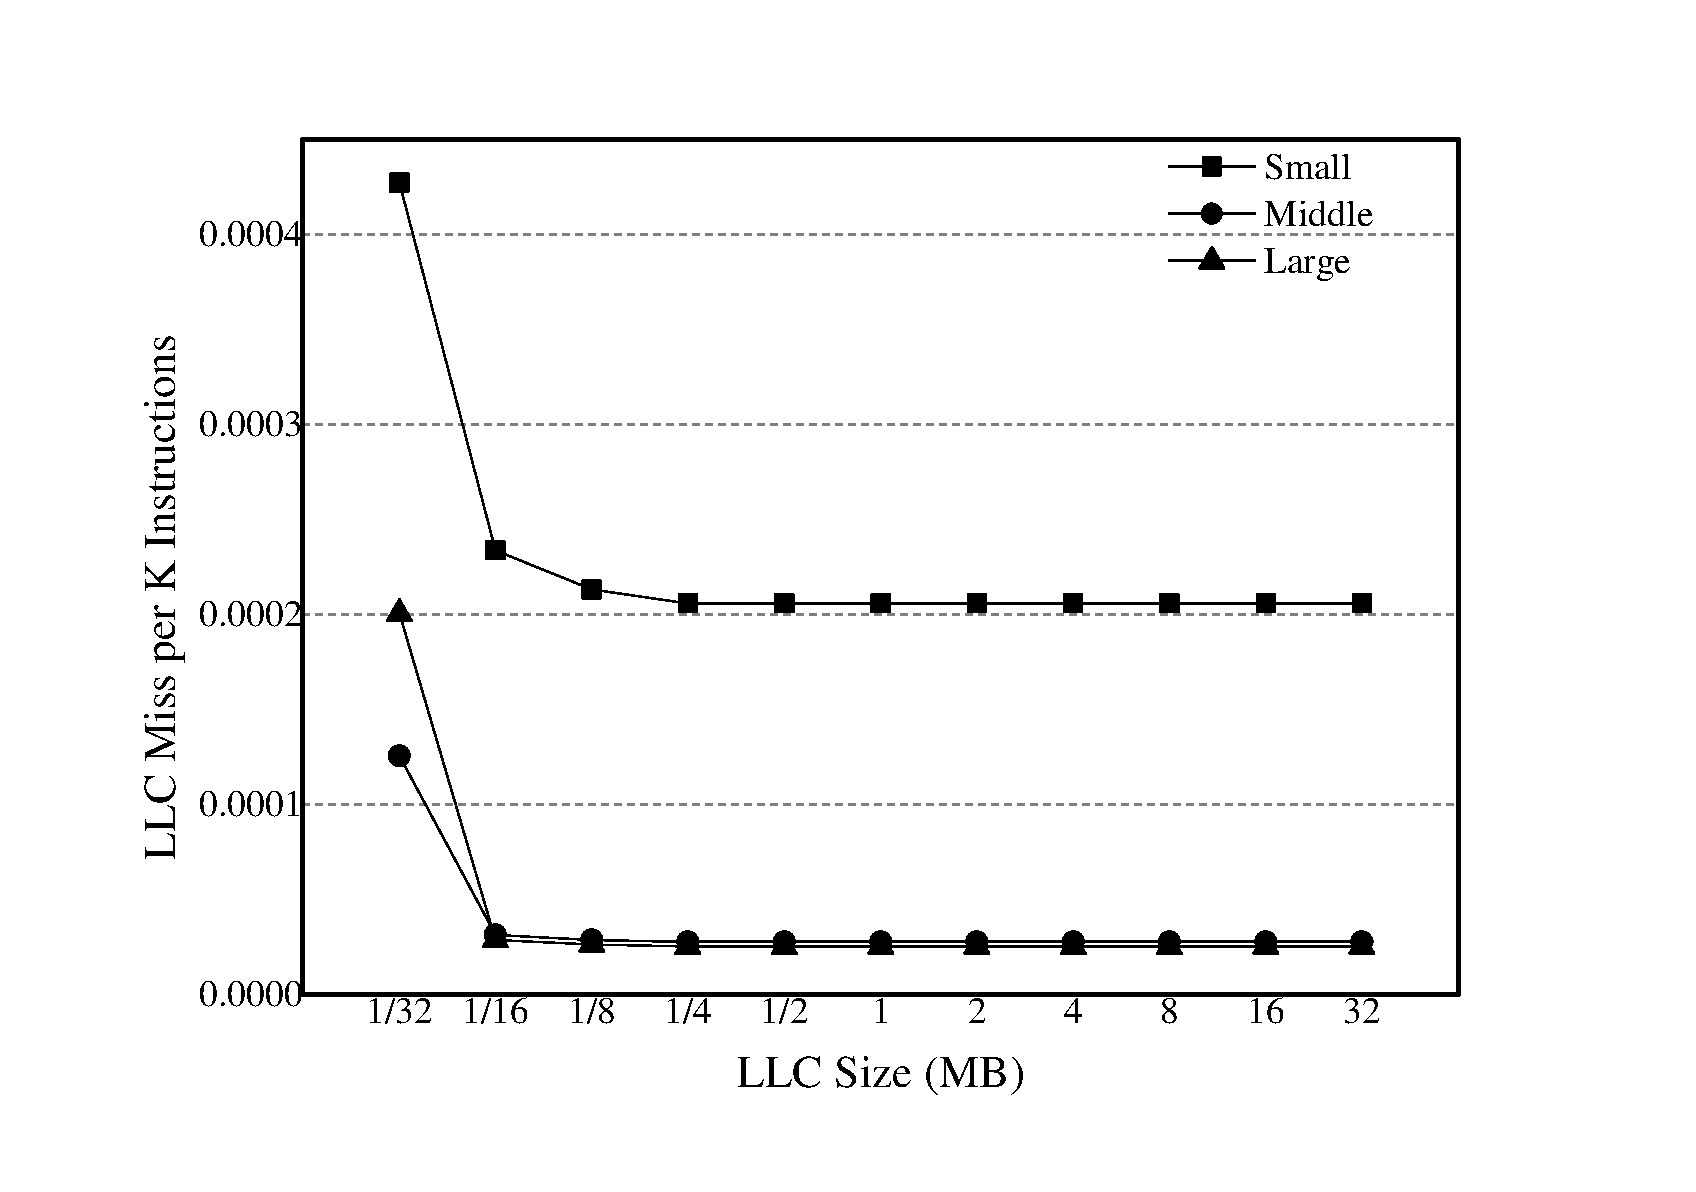
\includegraphics[width=0.50\textwidth]{graph/LLC_miss.pdf}
\caption{Last Level Cache Miss per K Instructions.}
\label{fig:LLC_miss}
\end{figure}

\subsection{Comparison of Two Versions}
\label{sec:comparison} 
The \SA solver involves a high percentage of floating point operations (FLOPs) while floating point units (FPUs) are one of the most energy-consuming units in modern processor's architecture. As is measure by Pin tool, the FLOP in \SA solver takes up about 10\% of the total instructions, thus it is necessary to research whether the FPU could be replaced by fixed-point units (totally or partially) in order to save the computation resource. 

In this experiment, I implement a fixed point version of \SA solver based on the floating point one and measure the differences between them in respect of accuracy and performance. 

The first topic we should discuss is the accuracy sacrifice of the fixed point version solver. The data file is chosen from the "Large" data sets (i.e. 1024 polynomial equations). Considering the average value of the resultant optimal points is about 5000, we set the threshold at 500. If the error range is larger than 500, we take this result is an "error". The error rate of different decimal bits is shown in Figure~\ref{fig:ER}. From the figure we could observe that the best decimal bit number is 6 with the smallest error rate of 8.4\%, which is still a high value when scientific computation is taken into consideration. As to Simulated Annealing, it takes cost functions in the form of polynomial equations and attempt to find the extreme point in given domains. Considering the simulation iteration is finite, the error threshold was set to 10\%, a solution would be marked "error" if exceeding the threshold. We take one thousand polynomial equations as an example, and the error rate is the proportion of error solutions. The high error rate of simulated annealing could be attributed to that the branch conditioner depends on a randomly-generated number which could change the expected interval in which locates the extreme point.

Furthermore, I examine the execution time of the two versions of which the result is plotted in Figure~\ref{fig:execution_time}. The speedup gained from substitution from floating point to fixed point is not as obvious as expected ($<=1.1$). Thus fixed point operation could not replace the FPU completely however partially substitution is acceptable when the requirement of accuracy is not very strict.  

\begin{figure}
\centering
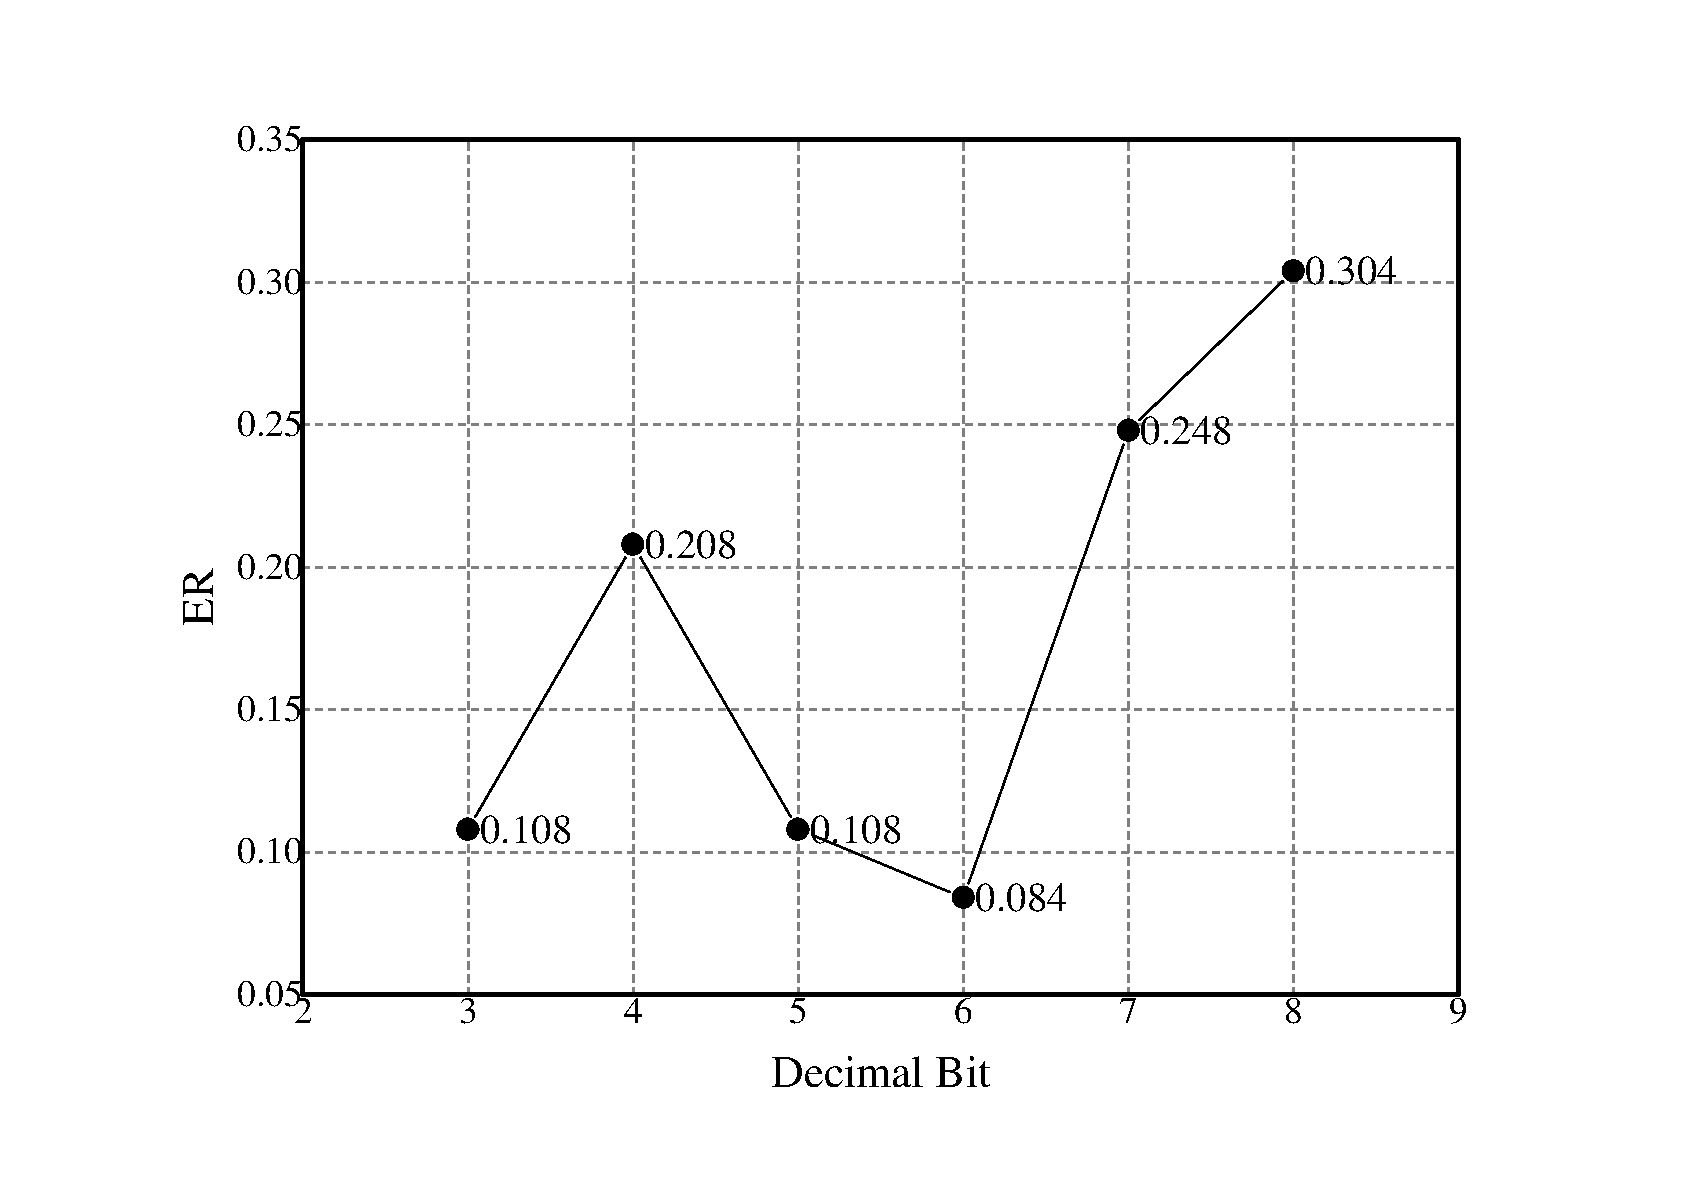
\includegraphics[width=0.50\textwidth]{graph/ER.pdf}
\caption{Error Rate of Results between Floating and Fixed Point Version.}
\label{fig:ER}
\end{figure}

\begin{figure}
\centering
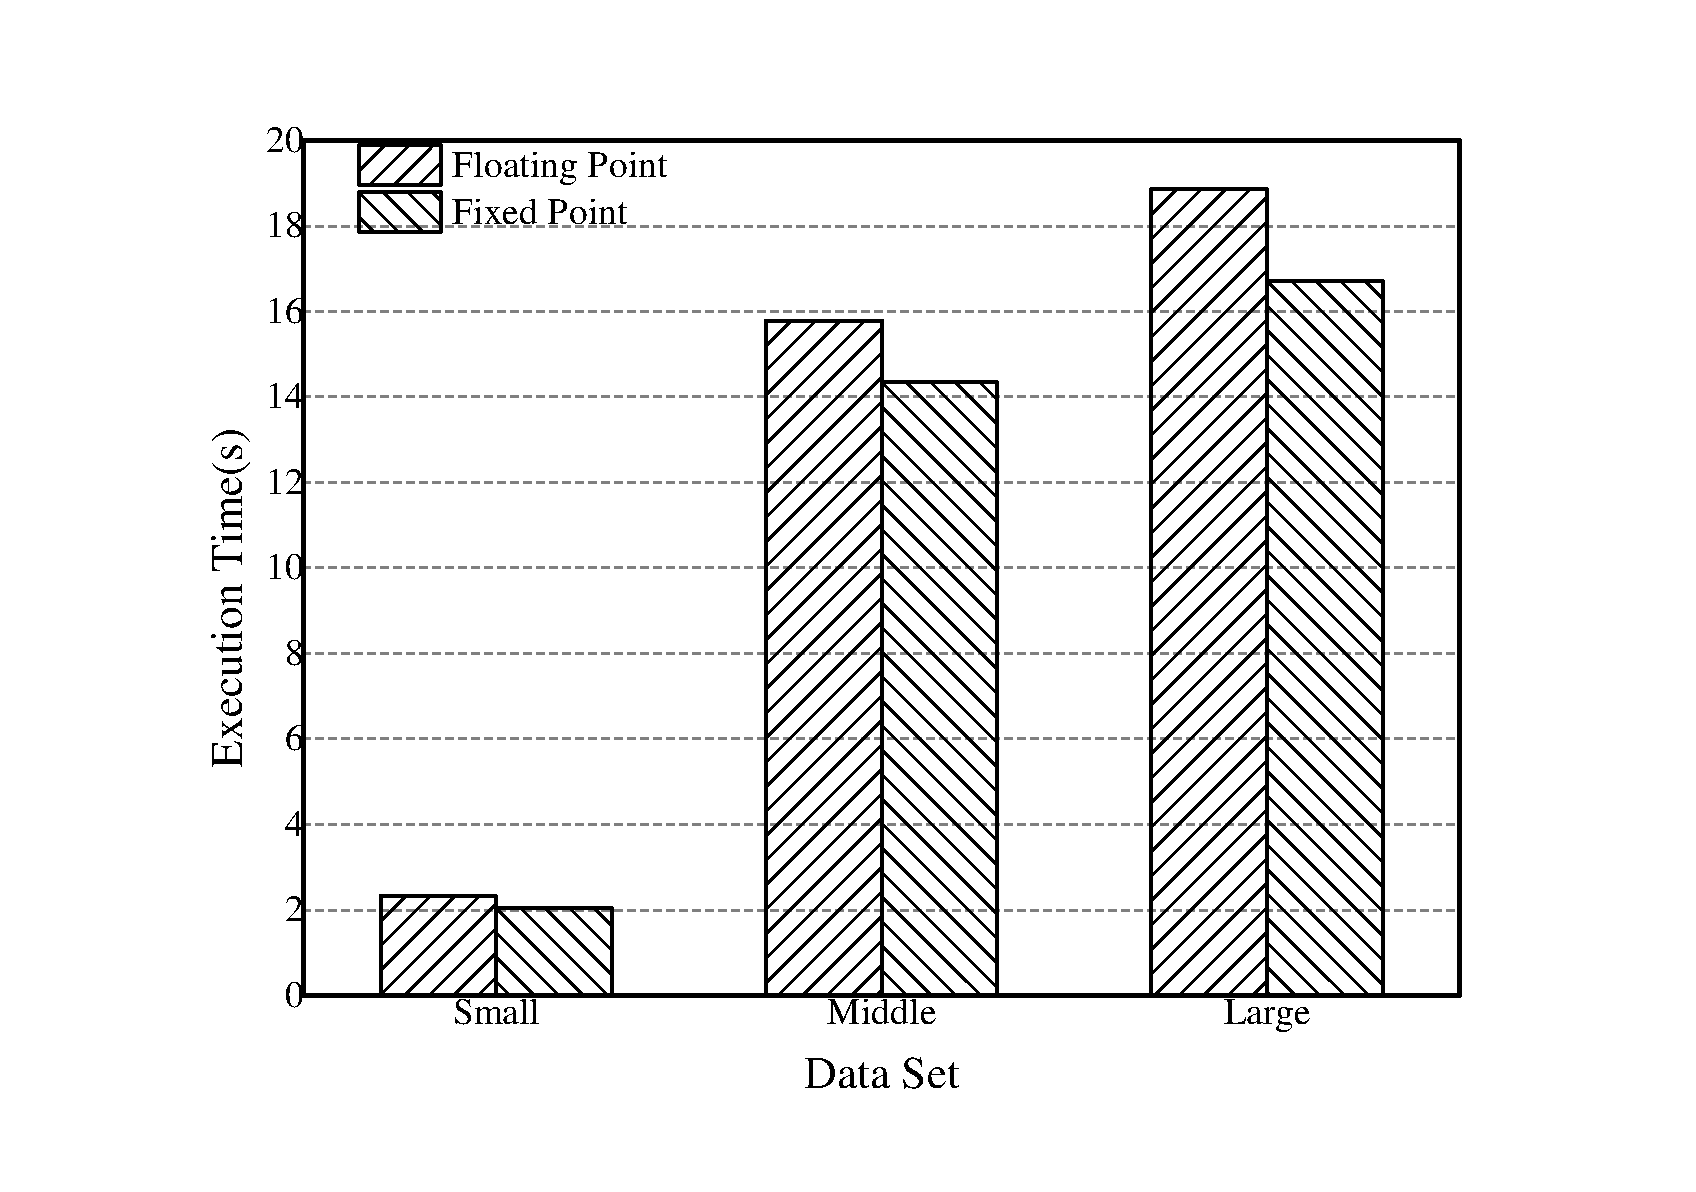
\includegraphics[width=0.50\textwidth]{graph/execution_time.pdf}
\caption{Execution Time of Floating and Fixed Point Version.}
\label{fig:execution_time}
\end{figure}

\section{Discussion}
\label{sec:discussion} 
As is analyzed in Section~\ref{sec:experiment}, the \SA solver is basically a computation-intensive program while the requirement on cache and memory is not very high when text-based input file is adopted. From the statistics we could get the following insights:
\begin{compactitem}
\item Memory and branch/call instructions are both important contributors to low pipeline fetch efficiency. Besides more sophisticated branch prediction strategy should be further explored in future work.
\item Low ILP and MLP value implies that the \SA solver could behave well using in-order processors, which could save much expense on chip placement.
\item Floating point operations could not be substituted completely by fixed point ones.
\item \SA solver is basically computation-intensive rather than memory-intensive. Clock frequency and the performance of on-chip cache are still fundamental factors.
\end{compactitem}  

\section{Conclusion and Future Work}
\label{sec:conclusion}


\section{Acknowledgements}
Thanks are due to our lecturer David Fagan who gave us a vivid and thought-provoking representation of natural computation topic and my tutor Prof. Zhang and my upperclassman Mr. Dai who gave me much precious help in primitive scientific research skills.

\bibliographystyle{abbrv}
\bibliography{biblio}

\end{document}

